\documentclass[a4paper,12pt,headsepline]{scrartcl}

%\part{title}
\usepackage[utf8]{inputenc}
\usepackage{graphicx}
\usepackage{caption,subcaption}
\usepackage[british]{babel}
\usepackage[T1]{fontenc}
\usepackage{geometry}
\usepackage{proof}
\geometry{left=3.5cm, right=2cm, top=2.5cm, bottom=2cm}
\usepackage{hyperref}
%\usepackage[hyphens,obeyspaces,spaces]{url}
\usepackage{fancybox}
\usepackage{amssymb,amsmath,amsthm}
\usepackage{gensymb}
\usepackage[linesnumbered,ruled,vlined,norelsize]{algorithm2e}
%\usepackage[bookmarksnumbered,pdftitle={\titleDocument},hyperfootnotes=false]{hyperref} 
\usepackage{color}
\usepackage{float}
\usepackage{enumerate}
\usepackage{tikz}

%test
%\usepackage[backend=bibtex]{biblatex}
%\usepackage{filecontents}

%\addbibresource{ref.bib}

\restylefloat{figure}

% Makros
%\newenvironment{sketch}{\begin{proof}[Proof (Sketch)]}{\end{proof}}
%\newtheorem{theorem}{Theorem}
%\newtheorem{assumption}{Assumption}
\newtheorem{lemma}{Lemma}
%\newtheorem{remark}{Remark}
%\newtheorem{definition}{Definition}
%\newtheorem{corollary}{Corollary}
\newcommand{\comment}[1]
{
  \begin{quotation}
    \textcolor{blue}{\underline{Edit:} #1}
  \end{quotation}
}
\newtheorem{aufgabe}{Exercise}
\newcommand{\Ex}[2]
{
	\setcounter{section}{#2}
	\section*{Übungsblatt #2 zu #1}
}
\newcommand{\TODO}[1]
{
  \begin{quotation}
    \textcolor{red}{\underline{TODO:} #1}
  \end{quotation}
}
% Zeichen 
\newcommand{\OO}{\ensuremath{\mathcal{O}}}
\newcommand{\ec}{\texttt{ec}}
\newcommand{\NP}{\call{NP}}
\newcommand{\call}[1]{\ensuremath{\mathcal{#1}}}

% neue Kopfzeilen mit fancypaket
\usepackage{fancyhdr} %Paket laden
\pagestyle{fancy} %eigener Seitenstil
\fancyhf{} %alle Kopf- und Fußzeilenfelder bereinigen
\fancyhead[L]{Benjamin \c Coban \\ Christoph Jabs}
\fancyhead[C]{Algorithmen und Komplexität \\ Blatt 2}
\fancyhead[R]{3526251 \\ 5567177}
\setlength{\headheight}{39pt}
\renewcommand{\headrulewidth}{0.4pt} %obere Trennlinie
%\fancyfoot[C]{\thepage} %Seitennummer
%\renewcommand{\footrulewidth}{0.4pt} %untere Trennlinie

\frenchspacing
\makeindex

% Pseudocode für Java
\usepackage{listings}
\lstset{numbers=left, numberstyle=\tiny, numbersep=5pt, keywordstyle=\color{black}\bfseries, stringstyle=\ttfamily,showstringspaces=false,basicstyle=\footnotesize,captionpos=b}
\lstset{language=java}

% Disable single lines at the start of a paragraph (Schusterjungen)
\clubpenalty = 10000
% Disable single lines at the end of a paragraph (Hurenkinder)
\widowpenalty = 10000
\displaywidowpenalty = 10000

\begin{document}

\begin{aufgabe}
\end{aufgabe}
\begin{enumerate}
	\item The \textit{neighbourhood} $N(S)$ of a set of vertices $S$ is a set of vertices, attached to any vertex $s\in S$. For a bipartite graph $G = (V_1 \cup V_2, E)$, the sets of vertices respect the property of bipartition when talking about Hall's Condition:
	\begin{align*}
	|N(S)| \geq |S| ~~~ S\subseteq V
	\end{align*}
	The following statement is to prove:
	\begin{align*}
	|N(S)| \geq |S| \forall (S\subseteq V_1 \vee S\subseteq V_2) \Leftrightarrow~G \text{ is perfectly matchable}
	\end{align*}
	\begin{proof}Since this is an equivalency, we have to argue for both directions of implication.
		\begin{itemize}
			\item[$\Rightarrow$] Hall's Condition holds for any subset of $V_1$ or $V_2$. Then, $|V_1| = |V_2|$. Otherwise, it would violate Hall's Condition since $N(V_1) = V_2$ and vice versa.\\
			Suppose, that there was a maximal but no perfect matching for $G$. Then, there is at least one unmatched vertex in $V_1$ and in $V_2$, since $|V_1| = |V_2|$. Suppose, this unmatched vertex $v$ is of degree 0 but then, Hall's Condition is violated since it has no neighbours. Every neighbour of $v$ is matched since the matching was maximal and $v$ is unmatched. Consider the alternating path starting from $v$ and since the matching was maximal, this path can not be augmented.  Let $S_1 \subseteq V_1, S_2\subseteq V_2$ be the vertices lying on the alternating paths. Then, $|S_1 - S_2| = 1$ since $v$ lies in either $V_1$ or $V_2$ and the rest is matched. Let without loss of generality $v\in V_1$, $S_2$ be the smaller set. Then $N(S_1) \subseteq S_2 < S_1$, contradicting Hall's Condition.
			\item[$\Leftarrow$] Let $M$ be a perfect matching for $G$. Consider any subset $S$ of $V_1$ or $V_2$. Then, the amount of neighbours of $S$ is at least as large as $S$ since there is a perfect matching, a match for every vertex of $S$.
		\end{itemize}
	\end{proof}
	\item For a bipartite graph $G = (V \cup W,E)$, the following holds:
	\begin{align}
		d(v) \geq 1 \wedge d(v) \geq d(w) \forall v\in V, w\in W, (u,w) \in E\label{eq:1}
	\end{align}
	Then, there exists a matching covering all vertices of $V$.
	\begin{proof}
		Let $|V| = n$. The size of $W$ depends on \ref{eq:1}. 
		\begin{align*}
		
		\end{align*}
		% Argue with the size of $W$ that you are able to remove vertices out of $W$ until Halls Condition is met - then, there will be a perfect matching and the statement is correct.
		% alternatively, write an algorithm and prove its correctness
	
	\end{proof}
\end{enumerate}
\newpage
\begin{aufgabe}
\end{aufgabe}

It is obvious that for $|M_i|\ge \frac{i}{i+1}|M^*|$ to hold for $i=1$, $|\mathcal P_1|\ge \frac 12 |M^*|$ needs to be true.
When starting to find the maximum set $\mathcal P_1$, there are two cases.
Either we start by adding an edge, which is in a maximum matching to $\mathcal P_1$ or we start by adding an edge which is not in such a maximum matching.
We will now look at these two cases.

\begin{enumerate}
    \item If the first edge we pick is in a maximum matching, then the maximum set of augmenting paths of length 1 is $M^*$ or another set of the same cardinality and therefore $|P_1|\ge \frac 12|M^*|$.
        Since in this case $|M_1|=|M^*|$, $|M_i|\ge \frac{i}{i+1}|M^*|$ is true for all $i$.
    \item 
\end{enumerate}

\newpage
\begin{aufgabe}
\end{aufgabe}

\begin{proof}
  We start with the following matching $M$ on the graph $G$, where the edges in the matching are marked red.

  \begin{center}
    \begin{tikzpicture}
      [ scale = .75
      , vertex/.style =
        { fill, circle }
      , free/.style =
        { blue }
      , edge/.style =
        { shorten >=5pt, shorten <=5pt, thick }
      , matched/.style =
        { red }
      ]
      \node [vertex] (0) at (-6, 6) {};
      \node [vertex] (1) at (-4, 6) {};
      \node [vertex,free] (2) at (-5, 5) {};
      \node [vertex] (3) at (-6, 4) {};
      \node [vertex] (4) at (-4, 4) {};
      \node [vertex] (5) at (-3, 3) {};
      \node [vertex] (6) at (-2, 4) {};
      \node [vertex] (7) at (-1, 3) {};
      \node [vertex] (8) at (-2, 2) {};
      \node [vertex] (9) at (-3, 1) {};
      \node [vertex] (10) at (-1, 1) {};
      \node [vertex] (11) at (0, 4) {};
      \node [vertex] (12) at (0, 6) {};
      \node [vertex] (13) at (2, 6) {};
      \node [vertex] (14) at (2, 4) {};
      \node [vertex] (15) at (1, 5) {};
      \node [vertex] (16) at (0, 0) {};
      \node [vertex] (17) at (2, 0) {};
      \node [vertex] (18) at (1, -1) {};
      \node [vertex] (19) at (0, -2) {};
      \node [vertex] (20) at (2, -2) {};
      \node [vertex] (21) at (-4, 0) {};
      \node [vertex] (22) at (-6, 0) {};
      \node [vertex] (23) at (-6, -2) {};
      \node [vertex] (24) at (-4, -2) {};
      \node [vertex,free] (25) at (-5, -1) {};
      \draw [edge,matched] (0.center) to (3.center);
      \draw [edge] (0.center) to (1.center);
      \draw [edge] (3.center) to (4.center);
      \draw [edge,matched] (4.center) to (1.center);
      \draw [edge] (2.center) to (1.center);
      \draw [edge] (0.center) to (2.center);
      \draw [edge] (3.center) to (2.center);
      \draw [edge] (2.center) to (4.center);
      \draw [edge] (4.center) to (5.center);
      \draw [edge,matched] (5.center) to (6.center);
      \draw [edge] (6.center) to (7.center);
      \draw [edge] (5.center) to (7.center);
      \draw [edge] (5.center) to (8.center);
      \draw [edge] (8.center) to (7.center);
      \draw [edge,matched] (9.center) to (8.center);
      \draw [edge] (5.center) to (9.center);
      \draw [edge] (9.center) to (10.center);
      \draw [edge] (10.center) to (7.center);
      \draw [edge] (8.center) to (10.center);
      \draw [edge] (21.center) to (9.center);
      \draw [edge] (22.center) to (21.center);
      \draw [edge,matched] (22.center) to (23.center);
      \draw [edge] (23.center) to (24.center);
      \draw [edge,matched] (24.center) to (21.center);
      \draw [edge] (22.center) to (25.center);
      \draw [edge] (25.center) to (24.center);
      \draw [edge] (23.center) to (25.center);
      \draw [edge] (25.center) to (21.center);
      \draw [edge,matched] (10.center) to (16.center);
      \draw [edge] (16.center) to (17.center);
      \draw [edge,matched] (17.center) to (20.center);
      \draw [edge] (16.center) to (19.center);
      \draw [edge] (19.center) to (20.center);
      \draw [edge,matched] (19.center) to (18.center);
      \draw [edge] (18.center) to (20.center);
      \draw [edge] (18.center) to (17.center);
      \draw [edge] (16.center) to (18.center);
      \draw [edge,matched] (7.center) to (11.center);
      \draw [edge] (12.center) to (11.center);
      \draw [edge] (11.center) to (14.center);
      \draw [edge] (11.center) to (15.center);
      \draw [edge] (15.center) to (13.center);
      \draw [edge] (12.center) to (15.center);
      \draw [edge,matched] (12.center) to (13.center);
      \draw [edge] (13.center) to (14.center);
      \draw [edge,matched] (15.center) to (14.center);
    \end{tikzpicture}
  \end{center}

  This matching is of size 12.
  From the lecture we know that a matching is maximum if there are no aufmenting paths in the graph, regarding the given matching.
  With the given matching, there are only two vertices left unmatched (marked blue), which means there is only one possibility where we could find an augmenting path.
  This path would need to connect the two free vertices and therefore pass through the middle part of the graph.
  We know focus on the middle part to proof that we cannot find an alternating path between the two green marked vertices.

  \begin{center}
    \begin{tikzpicture}
      [ scale = .75
      , vertex/.style =
        { fill, circle }
      , marked/.style =
        { green }
      , edge/.style =
        { shorten >=5pt, shorten <=5pt, thick }
      , matched/.style =
        { red }
      ]
      \node [vertex,marked] (4) at (-4, 4) {};
      \node [vertex] (5) at (-3, 3) {};
      \node [vertex] (6) at (-2, 4) {};
      \node [vertex] (7) at (-1, 3) {};
      \node [vertex] (8) at (-2, 2) {};
      \node [vertex] (9) at (-3, 1) {};
      \node [vertex] (10) at (-1, 1) {};
      \node [vertex,marked] (21) at (-4, 0) {};
      \draw [edge] (4.center) to (5.center);
      \draw [edge,matched] (5.center) to (6.center);
      \draw [edge] (6.center) to (7.center);
      \draw [edge] (5.center) to (7.center);
      \draw [edge] (5.center) to (8.center);
      \draw [edge] (8.center) to (7.center);
      \draw [edge,matched] (9.center) to (8.center);
      \draw [edge] (5.center) to (9.center);
      \draw [edge] (9.center) to (10.center);
      \draw [edge] (10.center) to (7.center);
      \draw [edge] (8.center) to (10.center);
      \draw [edge] (21.center) to (9.center);
    \end{tikzpicture}
  \end{center}

  It is quite easy to see that there is no alternating path between the two green vertices, since no single edge that is not in the matching connects the ends of the two edges in the matching.
  Therefore the graph with matching $M$ does not contain a augmenting path and $M$ of size 12 is maximum.

\end{proof}

\newpage
\begin{aufgabe}
\end{aufgabe}

\end{document}
